\documentclass{report}

\usepackage[utf8]{inputenc}
\usepackage{graphicx}
\usepackage[margin=35mm]{geometry}
\usepackage[colorlinks = true,linkcolor = red, urlcolor  = blue, citecolor = blue, anchorcolor = blue]{hyperref}
\usepackage[pagestyles]{titlesec}


\titleformat{\chapter}%
  {\normalfont\bfseries\LARGE}{\thechapter.}{10pt}{}

\titleformat{\section}%
  {\normalfont\bfseries\large}{\thesection.}{10pt}{}

\titleformat{\subsection}%
  {\normalfont\bfseries\small}{\thesubsection.}{10pt}{}



\title{Automatically defend from DoS and DDoS traffic flood attacks}
\author{Yinon Cohen and Maor Shabtay\\\\{ Advisor: Dr. Amit Dvir}\\\\{Ariel University}}

\date{October 2017}

\begin{document}
\maketitle

\tableofcontents
\addtocontents{toc}{~\hfill\textbf{Page}\par}


\newpage

\chapter {Introduction}
\hfill \break DoS and DDoS attacks are attempts to exhaust server side assets, and designed to prevent client-to-server communication (denial of service). These attacks aim to both public and private sectors, and occur more and more frequently. In addition, lately the massive DDoS attacks are performing 100 Gigabits per second, and being more common than ever. These attacks are sowing fear among organizations and private server owners.

\hfill \break Our project deals with understanding and examining DoS and DDoS attacks, and what are the solutions for them. In particularly, we will discuss and handle with traffic flood attacks on web servers, and will try to develop our own software or algorithm to block or to give any immediately pragmatic solution.

\hfill \break Our main goal is to develop an automatic system that would identify and analyze a traffic flood attack, defend the server from it, and in need - will block any IP or sub-net which the flood comes from. Our system should run on a CDN instead of on the server in order to save the server’s performances providing service
\hfill \break \hfill \break
    \begin{center}
        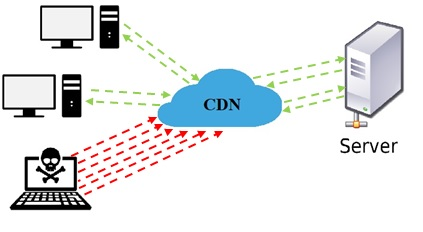
\includegraphics{pi}
    \end{center}
\newpage
\chapter {DoS and DDoS attacks}

\hfill \break DoS attacks are attempts to exhaust server-side assets and designed to prevent client-to-server communication (denial of service). Simply, we can say that stealth server sabotage wires or even the server is denial of service, but in the context of data security we discuss about remote attacks and not physical sabotaging.

\hfill \break DDoS attacks are very similar and sometimes even identical, and their intention is Distributed Denial of Service. In other words, the attack comes not from a single source, but from a large number of end stations – usually triggered by the attacker in the form of a king of virus located on these end stations. Most DDoS attacks are much more powerful and significant. It is important to understand that even an attack by two or three end stations is usually considered as a DoS attack, since there is really no significant flooding of the server.
\hfill \break Earlier this month Cisco released a white paper that is part of the company’s larger report, “Visual Networking Index Complete Forecast Update, 2015-2020.” Here are some statistics from that white paper, relevant to distributed denial of service (DDoS) attacks:
\begin{itemize}
\item Frequency of distributed denial-of-service (DDoS) attacks has increased more than 2.5 times over the last 3 years.
\item	The average size of DDoS attacks is increasing steadily and approaching 1 Gbps, enough to take most organizations completely off line.
\item	Peak DDoS attack size (Gbps) is increasing in a linear trajectory, with peak attacks reaching 300, 400, and 500 Gbps respectively, in 2013, 2014, and 2015, at about 10 to 15 percent per year.
\item	In 2015 the top motivation behind DDoS attacks was criminals demonstrating attack capabilities, with gaming and criminal extortion attempts in second and third place, respectively.
\item	DDoS attacks account for more than 5 percent of all monthly gaming-related traffic and more than 30 percent of gaming traffic while they are occurring.
\item	Globally the number of DDoS attacks grew 25 percent in 2015 and will increase 2.6-fold to 17 million by 2020.
\end{itemize}

\hfill \break The DoS and DDoS attacks can be divided into two types: 
\begin{itemize}
\item 	Attacks that flood and delay the service.
\item	Attacks that completely disrupt the service (and these we want to deal with in our project).

\end{itemize}
    \begin{center}
        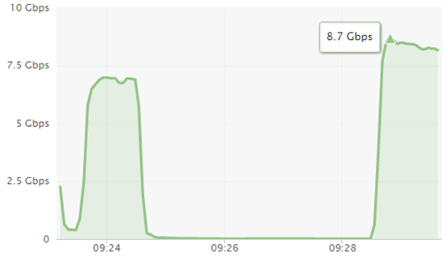
\includegraphics{ddos-attack-traffic-gbps}
    \end{center}


 \hfill \break
 \hfill \break We will now include both types of attacks for DoS and DDoS attacks in general, and we will divide the types into different main types, based on the seven-layer-model (OSI).



\section {DoS and DDoS over Application layer} 
 \hfill \break Attacks in the application layer are often generated by POST requests. They are also divided to sub protocols in the application layer – http / https.

\subsection {HTTP POST Flood} 
Creating and sending very large number of POST methods, to the extent that the server can't answer all requests, therefore service for real users of the server is compromised.

\subsection{HTTPS POST Flood} This is a flood of post methods that pass through SSL Session. The purpose of SSL is to take every message and decrypt it in order to inspect it. Flooding of these methods would harm the service.

\subsection {HTTP GET Flood} The attacker creates and sends to the server a huge amount of GET requests. The server needs to analyze all of them and return some data. Some people regard this attack as a Transport-layer attack, since sometimes the server would have to send a lot of data to the user \ attacker. Therefore, traffic and network bandwidth are flooded. Denial and service prevention depends on the server’s capacity to getting and sending back packets. If it is able to handle a huge number of requests – the traffic will be damaged, and if it fails, the requests that it receives from real users will not be handled as the server falls.

\subsection{HTTPS GET Flood} Overflow of GET requests on HTTPS protocol requires a lot of work from SSL Session – decryption every message and hence load and sabotage the service.
\hfill \break
\section {DoS and DDoS over Transport layer} 

 \hfill \break Flooding over Transport layer characterized mainly by packets that the server receives and is required to provide service – mostly by sending a requested data or any response packet.

 \subsection{Syn Flood} In this attack, the attacker takes advantage of the TCP principles that the server always wants to reach. When a server receives a Syn packet, it is a request from a client to open a connection, and it is obligated to respond to it and must return the client a Syn – Ack certificate. Each Syn message requires time from the server – analyzing the packet (understanding who created it, calculating ‘Check-sum’ etc.), and then be able to reply. Therefore, flooding these messages is slowing down and compromising the server’s serviceability.

\subsection{Rst Flood} Like Syn flood, the attacker takes advantage of TCP principles, including reliable communication. In case that a socket is closed or when one of the sides disconnected (and in few other situations), TCP has a solution. The connected side still wants to continue the communication (since there was no closing connection process), it sends a packet with a Rst flag and hence they have to re-open the connection. Like Syn packets overflowing, Rst packets overflowing also require a lot of work from the server and would sabotage the service.

\subsection{UDP Flood} UDP floods are used frequently for larger bandwidth DDoS attacks because they are connectionless and it is easy to generate UDP messages from many different scripting and compiled languages. The attack can be initiated by sending a large number of UDP packets to random ports. As a result, the server would check for the application listening at that port, realize that no one is and reply with ICMP packet saying ‘Destination Unreachable’. Thus, for a large number of UDP packets, the server will be forced into sending many ICMP packets and much performance.

\newpage
\section {DoS and DDoS over Network layer} 

 \hfill \break DoS and DDoS attacks over the Network layer are characterized with a large number of packets in order to overload the bandwidth and exhaust network resources. Network resources can be routers, firewalls and servers, and it is clear that their ability is final.

\subsection{ICMP Flood} ICMP protocol is typically used for error messages rather than data exchange between systems. Flooding messages with ICMP protocol – e.g. ping – is intended to overload the network.

 \hfill \break
\section {DoS and DDoS over Link layer}  

 \hfill \break DoS and DDoS attacks over the Network layer require access to the local network. Therefore, they are rare and more easy to detect.

\subsection{MAC Flood} A rare attack, in which the attacker has to be connected to the local switch. The attacker sends multiple dummy Ethernet frames, each with different invalid MAC address. Network switches maintaining their MAC table, and treating MAC addresses separately, and hence reserve some resources for each request. When all the memory in the table is used up, it either shuts down or becomes unresponsive.



 \hfill \break
\section {APDoS}

 \hfill \break APDoS is an attack that combines many DoS and DDoS attacks, and is carried out by a lot of hostile elements over time. APDoS represents the worst Denial of Service attack that can occur. The idea behind it is a combination of many attacks from multiple endpoints, and over long period of time, hence its name Advances Persistent DoS. In this attack, the attackers usually attack several stations in order to create a distraction from the DoS defenses, but concentrate on one main victim in the organization.


\chapter{DoS and DDoS defense solutions }




\section{DoS and DDoS solutions over Application layer}
 

\subsection {HTTP POST Flood}  There is a difficulty in distinguishing between legal traffic and attack.
The most effective mechanism that exists today is by combining methods of characterizing the movement of requests and identifying the source user.
When a random url is used, an exception check is required to understand that this was an attack and not an innocent use of the server. Part of the exception check is to try to identify the source user that triggers the attack, and you may notice that sometimes a large part of the package signature and content is the same.

\subsection {HTTPS Request Flood} Using the BIG-IP system and the F5 iRules scripting language.
Now available via the F5 DevCentral online community, this iRule states that if a device tries to renegotiate more than five times in any 60-second period, the connection is silently dropped.
The biggest benefit to this approach is that the attacker believes the attack is still working and in service, when in actuality, the server has ignored the request and moved on to processing valid user requests instead.


\subsection {HTTP GET Flood} Today We know about two detection algorithms, one is focusing on a browsing order of pages and the other is focusing on a correlation with browsing time to page information size. that implement detection techniques and evaluate attack detection rates, i.e., false positive and false negative. The results show that our techniques can detect the HTTP-GET flood attack effectively.


\section {DoS and DDoS solutions over Transport layer} 

\subsection{Syn Flood} We have a lot of solution for this attack:
Filtering ,Increasing Backlog,Reducing SYN-RECEIVED Timer,Recycling the Oldest Half-Open TCP,SYN Cache,SYN cookies,Hybrid Approaches,Firewalls and Proxies
We will expand a bit on SYN cookie is a technique used to resist SYN flood attacks. The technique's primary inventor Daniel J. Bernstein defines SYN cookies as "particular choices of initial TCP sequence numbers by TCP servers." In particular, the use of SYN cookies allows a server to avoid dropping connections when the SYN queue fills up. Instead, the server behaves as if the SYN queue had been enlarged. The server sends back the appropriate SYN+ACK response to the client but discards the SYN queue entry. If the server then receives a subsequent ACK response from the client, the server is able to reconstruct the SYN queue entry using information encoded in the TCP sequence number.

\subsection {Rst Flood}  Internet Protocol Security (IPsec) is a protocol suite for secure Internet Protocol (IP) communications that works by authenticating and encrypting each IP packet of a communication session. IPsec includes protocols for establishing mutual authentication between agents at the beginning of the session and negotiation of cryptographic keys to be used during the session. IPsec can be used in protecting data flows between a pair of hosts (host-to-host), between a pair of security gateways (network-to-network), or between a security gateway and a host (network-to-host). Internet Protocol security (IPsec) uses cryptographic security services to protect communications over Internet Protocol (IP) networks. IPsec supports network-level peer authentication, data origin authentication, data integrity, data confidentiality (encryption), and replay protection.

\section {DoS and DDoS solutions over Network layer} 

\subsection {ICMP Flood} Reconfiguring your perimeter firewall to disallow pings will block attacks originating from outside your network, albeit not internal attacks. Still, the blanket blocking of ping requests can have unintended consequences, including the inability to diagnose server issues.
The Incapsula DDoS protection provide blanket protection against ICMP floods by limiting the size of ping requests as well as the rate at which they can be accepted.

 \hfill \break

\section {APDoS solution}

 \hfill \break To combat APDoS, organizations require a single vendor, hybrid cyber security solution that protects networks and applications from a wide range of attacks. Ideally, such a solution includes all the different technologies needed for effective detection and mitigation, including DoS/DDoS protection, behavioral analysis, IPS, encrypted attack protection and web application firewall (WAF). Additionally, organizations also require new levels of partnership with their DDoS mitigation service provider and any ISP that provides managed DDoS services to coordinate for the effective detection and mitigation of a multi-vector assault.

\newpage


\chapter {Related Work}

\section {Traffic flooding attack detection with SNMP MIB using SVM}
 {\footnotesize  Jaehak Yu, Hansung Lee, Myung-Sup Kim *, Daihee Park}

Deep review of DoS and DDoS attacks, and rapid detection and proper response mechanisms, using MIB (Management Information base) over SNMP protocol.
[\href{http://www.sciencedirect.com/science/article/pii/S0140366408005094}{Link}]
  \hfill \break

\section {Change trend of averaged Hurst parameter of traffic under DDOS flood attacks}
 {\footnotesize Ming Li, School of Information Science and Technology, East China Normal University.}

Overview for the increasingly data traffic for a DoS and DDoS attack.
[\href{http://www.sciencedirect.com/science/article/pii/S0167404805001963}{Link}]
\hfill \break

\section{Software-Defined Networking (SDN) and Distributed Denial of Service (DDoS) Attacks in Cloud Computing Environments }
{\footnotesize Qiao Yan, F. Richard Yu, Senior Member, IEEE, Qingxiang Gong, and Jianqiang Li }

Advantages and disadvantages of using SDN as a traffic analyzer, centralized control and global view of the network. The article also represents studies of launching DDoS attack in SDN, as well as the methods against DDoS attack in SDN.
[\href{http://ieeexplore.ieee.org/abstract/document/7289347}{Link}]

\end{document}
